\documentclass[10pt, aspectratio=169]{beamer}

% --- PACKAGES DE BASE ---
\usepackage[utf8]{inputenc}
% Décommentez la ligne suivante si votre distribution LaTeX locale possède les polices EC (cm-super) :
% \usepackage[T1]{fontenc}
\usepackage[french]{babel}
\usepackage{amsmath, amssymb, amsfonts}
\usepackage{booktabs}
\usepackage{graphicx}
\usepackage{listings}
\usepackage{xcolor}
\usepackage{tikz}

% --- PALETTE DE COULEURS ÉLÉGANTE ---
% Bleu profond (primaire) et Vert d'eau/Teal (secondaire) pour une touche scientifique moderne
\definecolor{brandblue}{HTML}{1E3A8A}    % Navy Blue
\definecolor{brandteal}{HTML}{0D9488}    % Teal
\definecolor{darktext}{HTML}{1F2937}     % Anthracite
\definecolor{lightbg}{HTML}{F9FAFB}      % Gris très clair
\definecolor{codebg}{HTML}{F3F4F6}       % Fond de code gris neutre

% --- CONFIGURATION DU THÈME BEAMER ---
\usetheme{default}
\usecolortheme{default}

% Suppression des symboles de navigation obsolètes
\setbeamertemplate{navigation symbols}{}

% Couleurs globales
\setbeamercolor{structure}{fg=brandblue}
\setbeamercolor{normal text}{fg=darktext}
\setbeamercolor{background canvas}{bg=white}

% Style des titres de diapositive (Frametitle)
\setbeamercolor{frametitle}{fg=brandblue, bg=white}
\setbeamerfont{frametitle}{size=\large, series=\bfseries}
\setbeamertemplate{frametitle}{
    \nointerlineskip
    \begin{beamercolorbox}[wd=\paperwidth,ht=3.5ex,dp=1.5ex,leftskip=1cm]{frametitle}
        \insertframetitle
    \end{beamercolorbox}
    \vspace{-0.2cm}
    {\color{brandteal}\hrule height 1.5pt}
    \vspace{0.3cm}
}

% Pied de page personnalisé (Épuré et professionnel)
\setbeamertemplate{footline}{
    \leavevmode%
    \hbox{%
    \begin{beamercolorbox}[wd=.333333\paperwidth,ht=2.5ex,dp=1.125ex,center]{author in head/foot}%
        \usebeamerfont{author in head/foot}\insertshortauthor~~(\insertshortinstitute)
    \end{beamercolorbox}%
    \begin{beamercolorbox}[wd=.333333\paperwidth,ht=2.5ex,dp=1.125ex,center]{title in head/foot}%
        \usebeamerfont{title in head/foot}\insertshorttitle
    \end{beamercolorbox}%
    \begin{beamercolorbox}[wd=.333333\paperwidth,ht=2.5ex,dp=1.125ex,right]{date in head/foot}%
        \usebeamerfont{date in head/foot}\insertshortdate{}\hspace*{2em}
        \insertframenumber{} / \inserttotalframenumber\hspace*{2ex}
    \end{beamercolorbox}}%
    \vspace*{0pt}%
}
\setbeamercolor{author in head/foot}{fg=white, bg=brandblue}
\setbeamercolor{title in head/foot}{fg=white, bg=brandblue!90!black}
\setbeamercolor{date in head/foot}{fg=white, bg=brandblue!80!black}

% Style des blocs de texte
\setbeamercolor{block title}{bg=brandblue, fg=white}
\setbeamercolor{block body}{bg=lightbg, fg=darktext}
\setbeamercolor{block title example}{bg=brandteal, fg=white}
\setbeamercolor{block body example}{bg=lightbg, fg=darktext}

% Listes à puces
\setbeamertemplate{items}[circle]
\setbeamercolor{item}{fg=brandteal}
\setbeamercolor{subitem}{fg=brandblue}

% --- CONFIGURATION DE LISTINGS (CODE PYTHON MULTICOLORE) ---
\lstdefinestyle{pythonstyle}{
    backgroundcolor=\color{codebg},
    commentstyle=\color{gray},
    keywordstyle=\color{brandblue}\bfseries,
    numberstyle=\tiny\color{gray},
    stringstyle=\color{brandteal},
    basicstyle=\ttfamily\scriptsize,
    breakatwhitespace=false,
    breaklines=true,
    captionpos=b,
    keepspaces=true,
    numbers=left,
    numbersep=5pt,
    showspaces=false,
    showstringspaces=false,
    showtabs=false,
    tabsize=4,
    language=Python,
    frame=single,
    rulecolor=\color{brandblue!20},
    xleftmargin=10pt
}

% --- INFORMATIONS DU DIAPORAMA ---
\title[Soutenance de Stage]{Ajustement de surface de potentiels}
%\subtitle{Développement et optimisation de méthodes d'analyse physique}
\author[KADDOURI Amyne]{KADDOURI Amyne}
\institute[Univ. Rennes]{Université de Rennes \\ Master 1 Calcul Scientifique et Modélisation}
\date[20 Juillet 2026]{20 Juillet 2026}

\begin{document}

% 1. Slide de Titre (Épuré, sans éléments parasites)
\begin{frame}[plain]
    \titlepage
\end{frame}

% 2. Table des Matières (Sommaire)
\begin{frame}{Plan de la présentation}
    \tableofcontents[hideallsubsections]
\end{frame}

% -------------------------------------------------------------
% Section 1 : Contexte
% -------------------------------------------------------------
\section{Introduction \& Contexte}

\begin{frame}{Contexte théorique}
    \begin{itemize}
        \item \textbf{Système étudié :} Décrit par une fonction d'onde 
          $\Psi(\vec{r},\vec{\rho}) = F(\vec{r})\,\chi(\vec{\rho};\vec{r})$
        \item \textbf{Fonction d'onde :} Solution de l'équation de Schrödinger avec 
          \begin{itemize}
            \item $\vec{r}$ : position relative Atome - Molécule
            \item $\vec{\rho}$ : coordonnées internes de l'atome et de la molécule (électrons, etc.)
          \end{itemize}
    \end{itemize}
    
    \vspace{0.3cm}
   \begin{figure}
      \begin{center}
      \caption{Système Ar-HCN}\label{fig:Ar-HCN}
        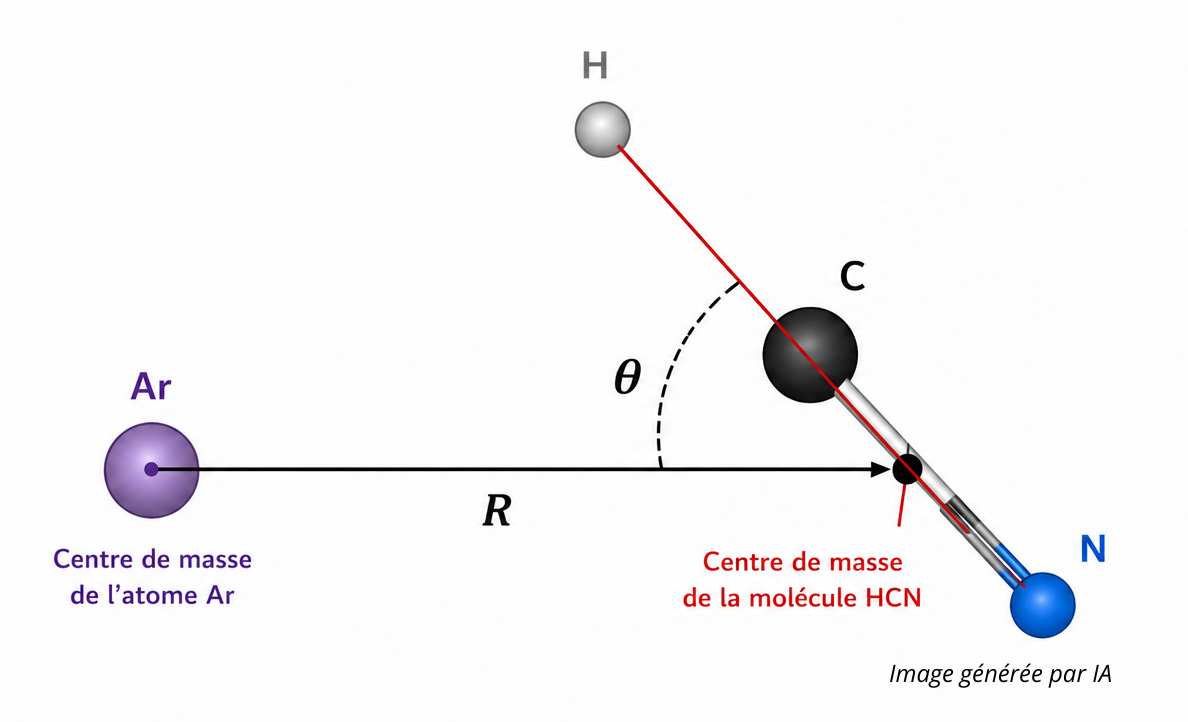
\includegraphics[width=0.45\textwidth]{../Figures/Soutenance/Systeme.png}
      \end{center}
    \end{figure}
     
    
\end{frame}


\begin{frame}{Sujet du Stage}

  \begin{exampleblock}{Références}
    \begin{itemize}
      \item Theoretical study of the He–HCN, Ne–HCN, Ar–HCN,
        and Kr–HCN complexes - 2000 - Rafał R. Toczyłowski, Fred Doloresco, and Sławomir M. Cybulski
      \item Autre article de Toczyłowski avec des paramètres pour chaque systèmes
  \end{itemize} 
  \end{exampleblock}
  
  \begin{block}{Objectifs}
  \begin{itemize}
    \item Calculer de nouveaux paramètres
    \item Déterminer comment évaluer leur qualité
    \item Comparaison des résultats
  \end{itemize}
\end{block}
 
\end{frame}


\begin{frame}{Le modèle physique}

\begin{center}
$\boxed{V(R,\theta)=V_{sh}(R,\theta)+V_{as}(R,\theta)}$
\end{center}


\begin{columns}[T]

%------------------ SHORT RANGE ------------------
\begin{column}{0.48\textwidth\small}

\begin{block}{Partie courte portée $V_{sh}$}

\[V_{sh}=G(R,\theta)e^{D(\theta)+B(\theta)R}\]

\begin{align*}
G(R,\theta)=\sum_{l=0}^{5}&
(g_{0,l}+g_{1,l}R+g_{2,l}R^2+g_{3,l}R^3)\\
&P_l(\cos\theta)
\end{align*}

\begin{center}
$D(\theta)=\sum\limits_{l=0}^{5}d_lP_l(\cos\theta)\;$
$\;B(\theta)=\sum\limits_{l=0}^{5}b_lP_l(\cos\theta)$
\end{center}
\begin{center}
\end{center}
\end{block}

\end{column}


%------------------ ASYMPTOTIC ------------------
\begin{column}{0.48\textwidth\small}

\begin{block}{Partie asymptotique $V_{as}$}

\begin{align*}
  V_{as}&=f_6(\lvert B(\theta)R\rvert)
  \frac{c_0P_0(\cos\theta)+c_2P_2(\cos\theta)}{R^6}\\
  &+f_7(\lvert B(\theta)R\rvert)\frac{c_1P_1(\cos\theta)+c_3P_3(\cos\theta)}{R^7}
\end{align*}

\[f_n(x)=1-e^{-x}\sum_{k=0}^{n}\frac{x^k}{k!}\]

\end{block}

\end{column}

\end{columns}

\end{frame}



% -------------------------------------------------------------
% Section 2 : implémentation
% -------------------------------------------------------------
\section{Implémentation du modèle}

\begin{frame}{Implémentation du modèle}
  \begin{block}{Etapes}
    \begin{itemize}
      \item Numérisation des tableaux de données
      \item Programmation de $V(R,\theta)$ utilisable et fonctionnelle
      \item Optimisation de $V$ pour de meilleures performances

    \end{itemize}
  \end{block}

  \begin{exampleblock}{Bibliothèques et fonctions utilisées}
    \begin{itemize}
      \item \texttt{numpy} / \texttt{math} : \texttt{cos, exp, radians, abs, ...}
      \item \texttt{scipy.special} : \texttt{eval\_legendre}, \texttt{factorial}
      \item \texttt{numpy.polynomial.legendre} : \texttt{legval}
    \end{itemize}
    
  \end{exampleblock}
  
\end{frame}

\begin{frame}{Implémentation plus performante}

  \begin{block}{Points d'amélioration de $V$}
    \begin{itemize}
      \item Vectorisation numpy
      \item Suppression de calculs inutiles
      \item Utilisation de fonctions Python plus performantes (ex : \texttt{legval})
    \end{itemize}
  \end{block}

  Tests des fonctions sur 500 valeurs de $R$ et $\theta$ aléatoires

  \begin{columns}[T]
    \begin{column}{0.48\textwidth}
        \begin{table}
        \caption{Différence $|V_{init} - V_{opt}|$ (en mEh)}\label{tab:diff}
          \begin{center}
            \begin{tabular}[c]{lll}
              \hline
              \multicolumn{1}{c}{Moyennne} & 
              \multicolumn{1}{c}{Max} &
              \multicolumn{1}{c}{e-type}\\
              \hline
              1.22e-08 & 1.79e-06 &1.09e-07\\
              \hline
            \end{tabular}
          \end{center}
        \end{table}
    \end{column}
    
    \begin{column}{0.48\textwidth}
      \begin{table}
        \caption{Temps d'execution moyen par appel}\label{tab:temps}
        \begin{center}
          \begin{tabular}[c]{|l|c|c|}
            \hline
            \multicolumn{1}{|c|}{\textbf{}} & 
            \multicolumn{1}{c}{$V_{init}$} & 
            \multicolumn{1}{c|}{$V_{opt}$} \\
            \hline
            100 appels & 3.12e-03s& 8.05e-04s\\
            50 least\_squares & 12.652s & 5.759s \\
            \hline
          \end{tabular}
        \end{center}
      \end{table}
    \end{column}
  \end{columns}
\end{frame}

% -------------------------------------------------------------
% Section 3 : Méthodes d'optimisation
% -------------------------------------------------------------
\section{Méthodes pour les fits de surface}

\begin{frame}[fragile]{Méthodes utilisées pour les ajustements de surface}
  
  \begin{center}
    Fonctions de la bibliothèque \texttt{scipy.optimize}
  \end{center}

  \begin{columns}[T]
    \begin{column}{0.33\textwidth\small}
      \begin{block}{\texttt{curve\_fit}}
        \begin{itemize}
          \item Ajustement de courbes 
          \item On entre des données (x,y)
          \item Cherche les paramètres qui approchent le mieux ces données
          \item Converge vers le minimum le plus proche de p0
        \end{itemize}
        
      \end{block}
    \end{column}

    \begin{column}{0.33\textwidth\small}
      \begin{exampleblock}{\texttt{least\_squares}}
        \begin{itemize}
          \item Plus générale que curve\_fit
          \item On fixe une fonction résidus
          \item Choix de bornes possible
          \item Converge vers le minimum le plus proche de p0
        \end{itemize}
        
      \end{exampleblock}
    \end{column}

    \begin{column}{0.33\textwidth\small}
      \begin{block}{\texttt{differential\_evolution}}
       \begin{itemize}
          \item Algorithme d'optimisation global 
          \item Ne nécessite pas de points de départ
          \item Méthode stochastique
          \item Echappe aux minimas locaux
          \item Plus lente

        \end{itemize} 
      \end{block}
    \end{column}
  \end{columns}

\end{frame}


% -------------------------------------------------------------
% Section 4 : Premier fit
% -------------------------------------------------------------

\section{Premiers ajustements de suface}

\begin{frame}{Premières données ab-initio}
  \begin{columns}[T]
    \begin{column}{0.45\textwidth}
      \begin{block}{}
        \begin{itemize}
          \item He-HCN : 138 points 
          \item Ne-HCN : 151 points 
          \item Ar-HCN : 140 points
        \end{itemize}
      \end{block}
      
      \begin{exampleblock}{}
        \begin{itemize}
          \item Plusieurs ajustements effectués avec différents paramètres d'entrée dans les fonctions
          \item Première selection graphique 
          \item Deuxième selection à l'aide des métriques : R², RMSE, MAE 
        \end{itemize}
      \end{exampleblock}
    \end{column}

    \begin{column}{0.45\textwidth}
      \begin{figure}
        \begin{center}
          \includegraphics[width=0.45\textwidth]{figures/}
        \end{center}
        \caption{}\label{fig:}
      \end{figure}
      
      
    \end{column}
  
  \end{columns}
   

\end{frame}

\begin{frame}[fragile]{Algorithme et Code Python (NumPy \& SciPy)}
    L'algorithme utilise la vectorisation de \textbf{NumPy} pour éviter les boucles lentes et la méthode d'intégration de Simpson via \textbf{SciPy}.

    \begin{lstlisting}[style=pythonstyle]
import numpy as np
from scipy.integrate import simpson

def compute_v_lambda(r, theta_grid, V_grid, lmbda):
    """
    Calcule le coefficient radial v_lambda(r) par quadrature numerique.
    """
    # Evaluation des polynomes de Legendre sur la grille angulaire
    P_l = np.polynomial.legendre.legval(np.cos(theta_grid), [0]*lmbda + [1])
    
    # Construction de l'integrande : V(r, theta) * P_lambda(cos(theta)) * sin(theta)
    integrand = V_grid * P_l * np.sin(theta_grid)
    
    # Integration par la methode de Simpson
    factor = (2 * lmbda + 1) / 2.0
    v_l = factor * simpson(y=integrand, x=theta_grid)
    return v_l
    \end{lstlisting}
\end{frame}

% -------------------------------------------------------------
% Section 4 : Résultats & Discussion
% -------------------------------------------------------------
\section{Résultats \& Analyse}

\begin{frame}{Analyse d'une Surface d'Énergie Potentielle (PES)}
    \begin{columns}[T]
        \begin{column}{0.5\textwidth}
            \textbf{Observations clés :}
            \begin{itemize}
                \item Présence d'un puits de potentiel prononcé à la distance d'équilibre $r_{\text{eq}}$.
                \item Précision de la projection de Legendre validée ($\epsilon < 10^{-4}$~cm$^{-1}$).
                \item \textbf{Performance :} Gain d'un facteur 50 par rapport à une implémentation Python pure.
            \end{itemize}
            \vspace{0.2cm}
            \begin{block}{Validation}
                Les résultats de l'interpolation s'accordent parfaitement avec les données de référence de la littérature.
            \end{block}
        \end{column}
        
        \begin{column}{0.48\textwidth}
            \centering
            \begin{tikzpicture}[scale=0.85]
                % Axes de coordonnées
                \draw[->, thick] (0,-2.2) -- (0,2.5) node[above] {$V(r)$ (cm$^{-1}$)};
                \draw[->, thick] (0,0) -- (4.5,0) node[right] {$r$ (\r{A})};
                
                % Tracé de la courbe de Morse (stable et ne cause pas d'explosion numérique)
                \draw[domain=0.5:4.2, smooth, variable=\x, brandblue, very thick] 
                    plot ({\x}, {3*(1 - exp(-1.5*(\x-1.25)))^2 - 2});
                
                % Lignes de repère
                \draw[dashed, gray] (1.25, -2) -- (1.25, 2.0) node[above] {$r_{\text{eq}}$};
                \draw[dashed, gray] (0, -2) -- (4.2, -2);
                \node[left, gray] at (0,-2) {$-D_e$};
                
                % Puits de potentiel
                \fill[brandteal] (1.25,-2) circle (3pt) node[below right] {Minimum};
            \end{tikzpicture}
            \vspace{0.2cm}
            \begin{center}
                \scriptsize\textcolor{brandblue!80}{\textbf{Figure 1 :} Coupe monodimensionnelle du potentiel d'interaction (potentiel de Morse).}
            \end{center}
        \end{column}
    \end{columns}
\end{frame}

% -------------------------------------------------------------
% Section 5 : Conclusion & Perspectives
% -------------------------------------------------------------
\section{Conclusion \& Perspectives}

\begin{frame}{Conclusion et Perspectives}
    \begin{block}{Bilan des Réalisations}
        \begin{itemize}
            \item \textbf{Fiabilité :} Conception d'une méthodologie d'interpolation spectrale performante.
            \item \textbf{Efficacité :} Optimisation de code Python pour le traitement de volumes de données massifs.
            \item \textbf{Outils :} Maîtrise d'un workflow Linux / Python Scientifique / Git.
        \end{itemize}
    \end{block}
    
    \vspace{0.3cm}
    
    \begin{block}{Perspectives de Recherche}
        \begin{itemize}
            \item Modélisation en 3D incluant des vibrations intra-moléculaires.
            \item Couplage direct de la PES optimisée avec des codes de collision quantique (méthode Close-Coupling).
        \end{itemize}
    \end{block}
\end{frame}

% 6. Slide de Fin (Remerciements)
\begin{frame}[plain]
    \vfill
    \centering
    \begin{beamercolorbox}[sep=12pt,center,rounded=true,shadow=false]{title}
        \usebeamerfont{title}\Large Merci de votre attention\\
    \end{beamercolorbox}
    \vfill
\end{frame}

\end{document}
